\documentclass[a4paper, 12pt]{article}

%% Language and font encodings
\usepackage[english]{babel}
\usepackage[utf8]{inputenc}
\usepackage[T1]{fontenc}

%% Sets page size and margins
\usepackage[a4paper,top=2cm,bottom=2cm,left=3cm,right=3cm,marginparwidth=1.75cm]{geometry}

%% Useful packages
\usepackage[tbtags]{amsmath}
\usepackage{mathtools}
\usepackage[colorlinks=true, allcolors=blue]{hyperref}
\usepackage{color}
\usepackage{caption}
\usepackage[shortlabels]{enumitem}
\usepackage{authblk}
\usepackage{xr}

% package to manage citations
\usepackage[backend=bibtex,style=authoryear-comp,sorting=nyt,isbn=false,url=false, natbib=true, doi=false]{biblatex}
\addbibresource{bibliography.bib}

\newcommand*\diff{\mathop{}\!\mathrm{d}}
%\newcommand{\argmax}[1]{\underset{#1}{\operatorname{arg}\,\operatorname{max}}\;}
\DeclareMathOperator{\argmax}{arg\,max}
\DeclarePairedDelimiter\abs{\lvert}{\rvert}%
\DeclarePairedDelimiter\norm{\lVert}{\rVert}%

\newcommand{\Hline}
{
\hline
\hline
}

\renewcommand{\thesection}{Web Appendix \Alph{section}}
\makeatletter
\renewcommand{\fnum@figure}{Web Figure \thefigure}
\makeatother

\AtBeginDocument{%
	\renewcommand{\thetable}{Web Table \arabic{table}}
}

\begin{document}
\title{\textbf{Supplementary Materials for ``Personalized Schedules for Burdensome Surveillance Tests''}}

\author[1,*]{\normalsize Anirudh Tomer}
\author[2,3]{Daan Nieboer}
\author[3]{Monique J. Roobol}
\author[2,4]{Ewout W. Steyerberg}
\author[1]{Dimitris Rizopoulos}
\affil[1]{Department of Biostatistics, Erasmus University Medical Center, the Netherlands}
\affil[2]{Department of Public Health, Erasmus University Medical Center, the Netherlands}
\affil[3]{Department of Urology, Erasmus University Medical Center, the Netherlands}
\affil[4]{Department of Biomedical Data Sciences, Leiden University Medical Center, the Netherlands}
\affil[ ]{*\textit {email}: a.tomer@erasmusmc.nl}

\date{}

\maketitle

% !TEX root =  ../supplementary.tex

\section{Joint Model for Time to Event and Longitudinal Outcomes}
\label{web_sec : jm_framework}
We start with the definition of the joint modeling framework that will be used to fit a model to the available dataset, and then to plan biopsies for future patients. Let $T_i^*$ denote the true Gleason reclassification (referred to as GR hereafter) time for the $i$-th patient enrolled in an AS program. Let $S$ be the schedule of biopsies prescribed to this patient. The corresponding vector of time of biopsies is denoted by $T_i^S = \{T^S_{i0}, T^S_{i1}, \ldots, T^S_{i{N_i^S}}; T^S_{ij} < T^S_{ik}, \forall j<k\}$, where $N_i^S$ are the total number of biopsies conducted. Because of the periodical nature of biopsy schedules, $T_i^*$ cannot be observed directly and it is only known to fall in an interval $(l_i, r_i]$, where $l_i = T^S_{i{N_i^S - 1}}, r_i = T^S_{i{N_i^S}}$ if GR is observed, and $l_i = T^S_{i{N_i^S}}, r_i=\infty$ if GR is not observed yet. Further let $\bmath{y}_i$ denote the $n_i \times 1$  vector of PSA levels for the $i$-th patient. For a sample of $n$ patients the observed data is denoted by $\mathcal{D}_n = \{l_i, r_i, \bmath{y}_i; i = 1, \ldots, n\}$.

The longitudinal outcome of interest, namely PSA level, is continuous in nature and thus to model it the joint model utilizes a linear mixed effects model (LMM) of the form:
\begin{equation*}
\begin{split}
y_i(t) &= m_i(t) + \varepsilon_i(t)\\
&=\bmath{x}_i^T(t) \bmath{\beta} + \bmath{z}_i^T(t) \bmath{b}_i + \varepsilon_i(t),
\end{split}
\end{equation*}
where $\bmath{x}_i(t)$ denotes the row vector of the design matrix for fixed effects and $\bmath{z}_i(t)$ denotes the same for random effects. Correspondingly the fixed effects are denoted by $\bmath{\beta}$ and random effects by $\bmath{b}_i$. The random effects are assumed to be normally distributed with mean zero and $q \times q$ covariance matrix $\bmath{D}$. The true and unobserved PSA level at time $t$ is denoted by $m_i(t)$. Unlike $y_i(t)$, the former is not contaminated with the measurement error $\varepsilon_i(t)$. The error is assumed to be normally distributed with mean zero and variance $\sigma^2$, and is independent of the random effects $\bmath{b}_i$.

To model the effect of PSA on hazard of GR, joint models utilize a relative risk sub-model. The hazard of GR for patient $i$ at any time point $t$, denoted by $h_i(t)$, depends on a function of subject specific linear predictor $m_i(t)$ and/or the random effects:
\begin{align*}
h_i(t \mid \mathcal{M}_i(t), \bmath{w}_i) &= \lim_{\Delta t \to 0} \frac{\mbox{Pr}\big\{t \leq T^*_i < t + \Delta t \mid T^*_i \geq t, \mathcal{M}_i(t), \bmath{w}_i\big\}}{\Delta t}\\
&=h_0(t) \exp\big[\bmath{\gamma}^T\bmath{w}_i + f\{M_i(t), \bmath{b}_i, \bmath{\alpha}\}\big], \quad t>0,
\end{align*}
where $\mathcal{M}_i(t) = \{m_i(v), 0\leq v \leq t\}$ denotes the history of the underlying PSA levels up to time $t$. The vector of baseline covariates is denoted by $\bmath{w}_i$, and $\bmath{\gamma}$ are the corresponding parameters. The function $f(\cdot)$ parametrized by vector $\bmath{\alpha}$ specifies the functional form of PSA levels \citep{brown2009assessing,rizopoulos2012joint,taylor2013real,rizopoulos2014bma} that is used in the linear predictor of the relative risk model. Some functional forms relevant to the problem at hand are the following: 
\begin{eqnarray*}
\left \{
\begin{array}{l}
f\{M_i(t), \bmath{b}_i, \bmath{\alpha}\} = \alpha m_i(t),\\
f\{M_i(t), \bmath{b}_i, \bmath{\alpha}\} = \alpha_1 m_i(t) + \alpha_2 m'_i(t),\quad \text{with}\  m'_i(t) = \frac{\rmn{d}{m_i(t)}}{\rmn{d}{t}}.\\
\end{array}
\right.
\end{eqnarray*}
These formulations of $f(\cdot)$ postulate that the hazard of GR at time $t$ may be associated with the underlying level $m_i(t)$ of the PSA at $t$, or with both the level and velocity $m'_i(t)$ of the PSA at $t$. Lastly, $h_0(t)$ is the baseline hazard at time $t$, and is modeled flexibly using P-splines. More specifically:
\begin{equation*}
\log{h_0(t)} = \gamma_{h_0,0} + \sum_{q=1}^Q \gamma_{h_0,q} B_q(t, \bmath{v}),
\end{equation*}
where $B_q(t, \bmath{v})$ denotes the $q$-th basis function of a B-spline with knots $\bmath{v} = v_1, \ldots, v_Q$ and vector of spline coefficients $\gamma_{h_0}$. To avoid choosing the number and position of knots in the spline, a relatively high number of knots (e.g., 15 to 20) are chosen and the corresponding B-spline regression coefficients $\gamma_{h_0}$ are penalized using a differences penalty \citep{eilers1996flexible}. 

\subsection{Parameter Estimation}
We estimate parameters of the joint model using Markov chain Monte Carlo (MCMC) methods under the Bayesian framework. Let $\bmath{\theta}$ denote the vector of the parameters of the joint model. The joint model postulates that given the random effects, time to GR and longitudinal responses taken over time are all mutually independent. Under this assumption the posterior distribution of the parameters is given by:
\begin{align*}
p(\bmath{\theta}, \bmath{b} \mid \mathcal{D}_n) & \propto \prod_{i=1}^n p(l_i, r_i, \bmath{y}_i \mid \bmath{b}_i, \bmath{\theta}) p(\bmath{b}_i \mid \bmath{\theta}) p(\bmath{\theta})\\
& \propto \prod_{i=1}^n p(l_i, r_i \mid \bmath{b}_i, \bmath{\theta}) p(\bmath{y_i} \mid \bmath{b}_i, \bmath{\theta}) p(\bmath{b}_i \mid \bmath{\theta}) p(\bmath{\theta}),\\
p(\bmath{b}_i \mid \bmath{\theta}) &= \frac{1}{\sqrt{(2 \pi)^q \text{det}(\bmath{D})}} \exp(\bmath{b}_i^T \bmath{D}^{-1} \bmath{b}_i),
\end{align*}
where the likelihood contribution of longitudinal outcome conditional on random effects is:
\begin{align*}
p(\bmath{y_i} \mid \bmath{b}_i, \bmath{\theta}) &= \frac{1}{\big(\sqrt{2 \pi \sigma^2}\big)^{n_i}} \exp\bigg(-\frac{{\lVert{\bmath{y_i} - \bmath{X}_i\bmath{\beta} - \bmath{Z}_i\bmath{b}_i}\rVert}^2}{\sigma^2}\bigg),\\
\bmath{X}_i &= \{\bmath{x}_i(t_{i1})^T, \ldots, \bmath{x}_i(t_{in_i})^T\}^T,\\
\bmath{Z}_i &= \{\bmath{z}_i(t_{i1})^T, \ldots, \bmath{z}_i(t_{in_i})^T\}^T.
\end{align*}
The likelihood contribution of the time to GR outcome is given by:
\begin{equation}
\label{web_eq : likelihood_contribution_survival}
p(l_i,r_i\mid \bmath{b}_i,\bmath{\theta}) = \exp\Big\{-\int_0^{l_i} h_i(s \mid \mathcal{M}_i(s), \bmath{w}_i)\rmn{d}{s}\Big\} - \exp\Big\{-\int_0^{r_i}h_i(s \mid \mathcal{M}_i(s), \bmath{w}_i)\rmn{d}{s}\Big\}.
\end{equation}
The integral in (\ref{web_eq : likelihood_contribution_survival}) does not have a closed-form solution, and therefore we use a 15-point Gauss-Kronrod quadrature rule to approximate it.

We use independent normal priors with zero mean and variance 100 for the fixed effects $\bmath{\beta}$, and inverse Gamma prior with shape and rate both equal to 0.01 for the parameter $\sigma^2$. For the variance-covariance matrix $\bmath{D}$ of the random effects we take inverse Wishart prior with an identity scale matrix and degrees of freedom equal to $q$ (number of random effects). For the relative risk model's parameters $\bmath{\gamma}$ and the association parameters $\bmath{\alpha}$, we use a a global-local ridge-type shrinkage prior. For example, for the $s$-{th} element of $\bmath{\alpha}$ we assume (similarly for $\bmath{\gamma}$):
\begin{equation*} 
\alpha_s \sim \mathcal{N}(0, \tau\psi_s), \quad \tau^{-1} \sim \mbox{Gamma}(0.1, 0.1),  \quad \psi_s^{-1} \sim \mbox{Gamma}(1, 0.01).
\end{equation*} 
The global smoothing parameter $\tau$ has sufficiently mass near zero to ensure shrinkage, while the local smoothing parameter $\psi_s$ allows individual coefficients to attain large values. For the penalized version of the B-spline approximation to the baseline hazard, we use the following prior for parameters $\gamma_{h_0}$ \citep{lang2004bayesian}:
\begin{equation*}
p(\gamma_{h_0} \mid \tau_h) \propto \tau_h^{\rho(\bmath{K})/2} \exp\bigg(-\frac{\tau_h}{2}\gamma_{h_0}^T \bmath{K} \gamma_{h_0}\bigg),
\end{equation*}
where $\tau_h$ is the smoothing parameter that takes a Gamma(1, 0.005) hyper-prior in order to ensure a proper posterior for $\gamma_{h_0}$, $\bmath{K} = \Delta_r^T \Delta_r + 10^{-6} \bmath{I}$, where $\Delta_r$ denotes the $r$-th difference penalty matrix, and $\rho(\bmath{K})$ denotes the rank of $\bmath{K}$.
\clearpage
% !TEX root =  ../supplementary.tex

\section{Fitting the Joint Model to the PRIAS Dataset}
\label{sec : param_estimates_jm_fit_prias}
For each of the PRIAS patients, we know their age at the time of inclusion in AS, PSA history and the time interval in which GR is detected. PSA was measured at every three months for the first two years and every six months thereafter. For the longitudinal analysis of PSA we use $\log_2 \mbox{PSA}$ measurements instead of the raw data \citep{nieboer2015nonlinear}. The longitudinal sub-model of the joint model we fit is given by:
\begin{equation}
\label{eq : long_model_prias_web}
\begin{aligned}
\log_2 \mbox{PSA}_i(t) &= \beta_0 + \beta_1 (\mbox{Age}_i-70) + \beta_2 (\mbox{Age}_i-70)^2 + \sum_{k=1}^4 \beta_{k+2} B_k(t,\mathcal{K})\\ 
&+  b_{i0} + b_{i1} B_7(t, 0.1) + b_{i2} B_8(t, 0.1) +
\varepsilon_i(t),
\end{aligned}
\end{equation}
where $B_k(t, \mathcal{K})$ denotes the $k$-th basis function of a B-spline with three internal knots at $\mathcal{K} =\{0.1, 0.5, 4\}$ years, and boundary knots at zero and seven (0.99 quantile of the observed follow-up times) years. The spline for the random effects consists of one internal knot at 0.1 years and boundary knots at zero and seven years. Age of patients was median centered to avoid numerical instabilities during parameter estimation. The error $\varepsilon_i(t)$ is assumed to be t-distributed with three degrees of freedom and scale $\sigma$, and is independent of the random effects $\bmath{b}_i$. For the relative risk sub-model the hazard function we fit is given by:
\begin{equation}
\label{eq : hazard_prias_web}
h_i(t) = h_0(t) \exp\big\{\gamma_1 (\mbox{Age}_i-70)  + \gamma_2 (\mbox{Age}_i-70)^2 + \alpha_1 m_i(t) + \alpha_2 m'_i(t)\big\},
\end{equation}
where $\alpha_1$ and $\alpha_2$ are measures of strength of the association between hazard of GR and $\log_2 \mbox{PSA}$ value $m_i(t)$ and $\log_2 \mbox{PSA}$ velocity $m'_i(t)$, respectively.

\subsection{Choice of the t-distribution for the Error Term}
\label{subsec : t_dist_choice}
For the error term $\varepsilon_i(t)$ in the longitudinal sub-model we assumed a t-distribution with three degrees of freedom and scale $\sigma$. This decision was taken on the basis of quantile-quantile plot (left panel of Web Figure \ref{fig : qqplot_norm_t3_web}) of the residuals from a joint model fitted to the PRIAS dataset in which errors were assumed to be normally distributed with mean zero and variance $\sigma^2$. It can be seen that the residuals from this model exhibit symmetric long tails. We thank the Referees for motivating us to inspect this in detail. In this regard, we then fitted two more joint models, each with errors assumed to be t-distributed with four and three degrees of freedom. Based on the quantile-quantile plots, the model we eventually selected was the one in which t-distribution had three degrees freedom. The quantile-quantile plot for this model is shown in the right panel of Web Figure \ref{fig : qqplot_norm_t3_web}.

\begin{figure}[!htb]
\centerline{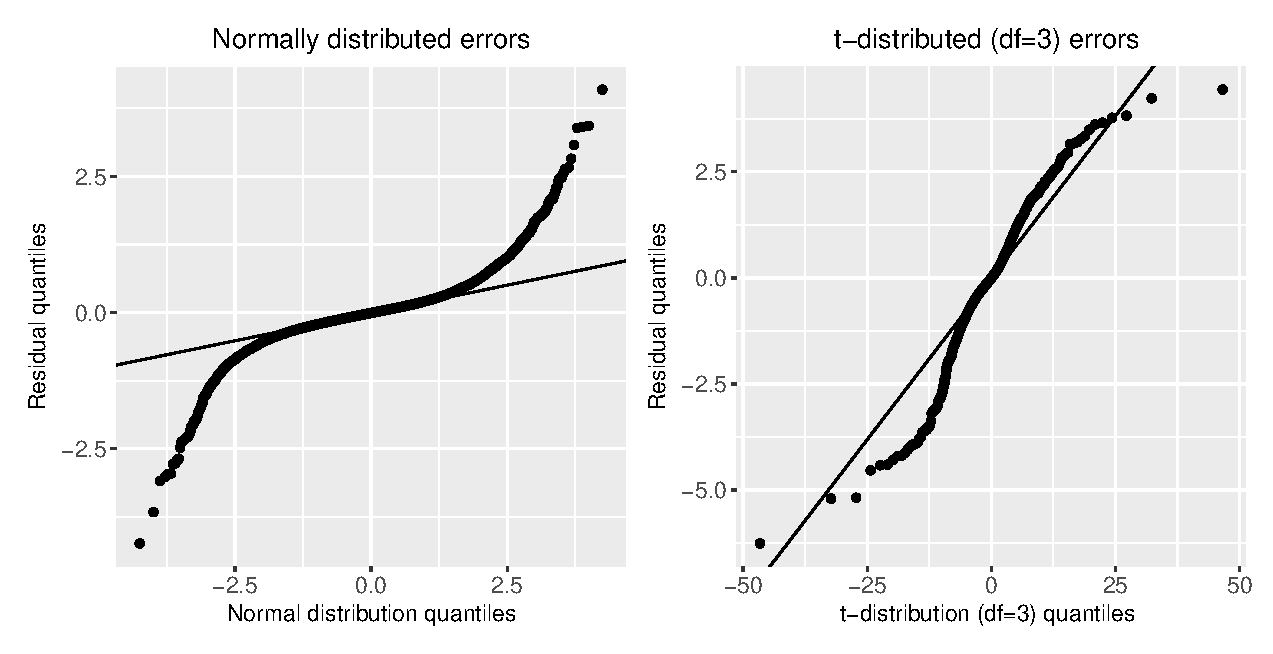
\includegraphics[width=\columnwidth]{images/model_fit/qqplot_norm_t3.eps}}
\caption{Quantile-quantile plots of subject specific residuals obtained from joint models with assumption of normally distributed errors, and t-distributed (df=3) errors, fitted to the PRIAS data set.}
\label{fig : qqplot_norm_t3_web}
\end{figure}

\clearpage

\subsection{Parameter Estimates}
\label{subsec : param_estimates}
The posterior parameter estimates for the joint model we fitted to the PRIAS dataset are shown in \ref{tab : PSA_long} (longitudinal sub-model) and \ref{tab : PSA_survival} (relative risk sub-model), and parameter estimates for the variance-covariance matrix from the longitudinal sub-model are the following:
\begin{equation*}
\bmath{D} = \begin{bmatrix}
       0.469 & 0.092 & -0.099 \\[0.3em]
       0.092 & 1.092 & 0.378 \\[0.3em]
       -0.099 & 0.378 & 0.898
     \end{bmatrix}
\end{equation*} 
For longitudinal sub-model parameter estimates, in \ref{tab : PSA_long} we can see that the age of the patient trivially affects the baseline $\log_2 \mbox{PSA}$ score. Since the longitudinal evolution of $\log_2 \mbox{PSA}$ is modeled with non-linear terms, the interpretation of the coefficients corresponding to time is not straightforward. In lieu of the interpretation, in Web Figure \ref{fig : fitted_trend_psa} we present the fitted marginal evolution of $\log_2 \mbox{PSA}$ over a period of 10 years for a hypothetical patient who was included in AS at the age of 70 years. In addition we present plots of observed versus fitted profiles for nine randomly selected patients (each with more than 3 observations) in Web Figure \ref{fig : subject_fittedVsObserved_psa_t3}.

\begin{figure}[!htb]
\centerline{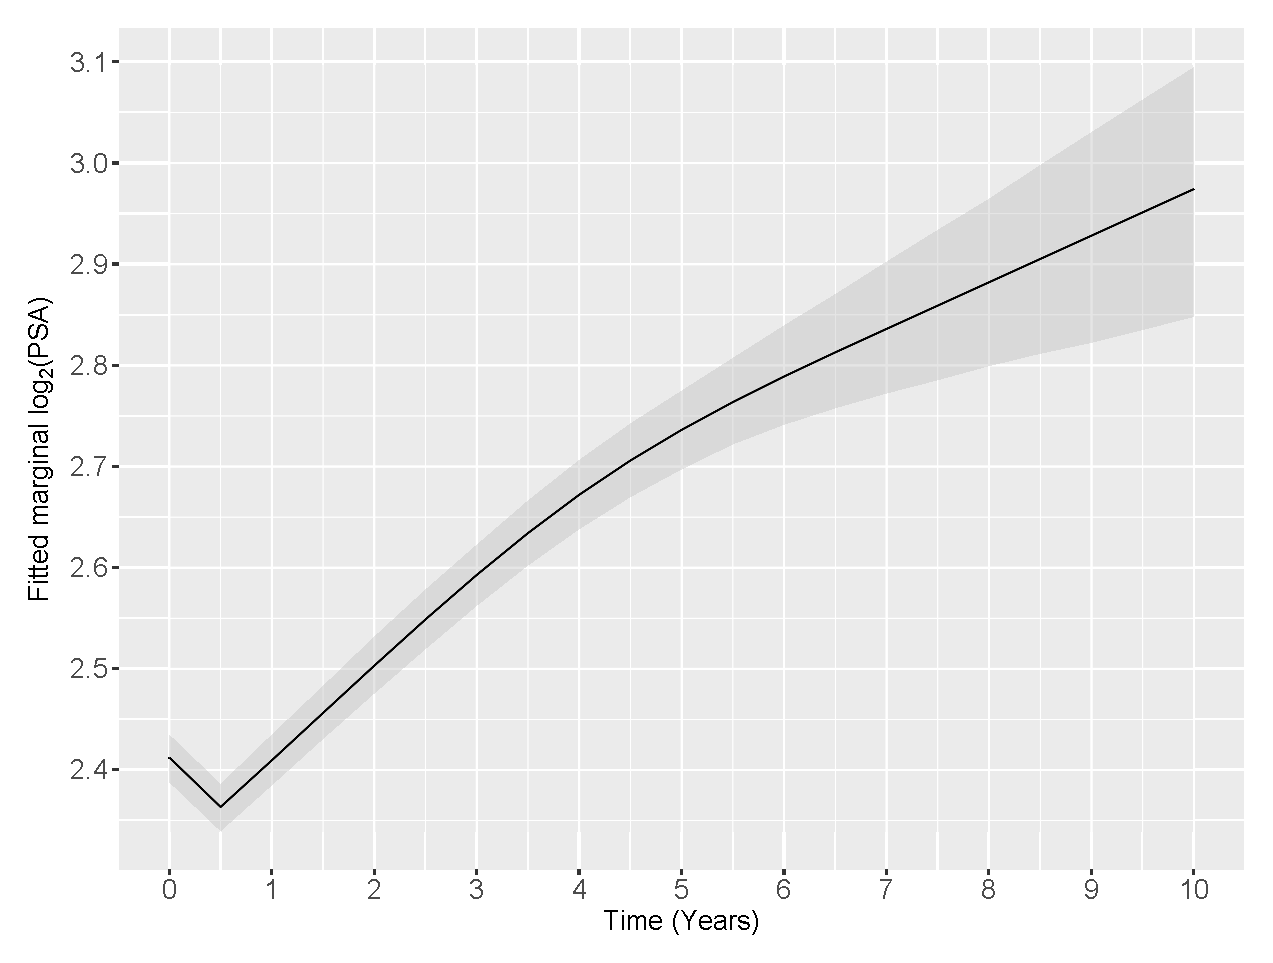
\includegraphics[width=\columnwidth]{images/model_fit/marginal_fitted_psa_t3.eps}}
\caption{Fitted marginal evolution of $\log_2 \mbox{PSA}$ over a period of 10 years with 95\% credible interval, for a hypothetical patient who was included in AS at the age of 70 years.}
\label{fig : fitted_trend_psa}
\end{figure}

\begin{figure}[!htb]
	\centerline{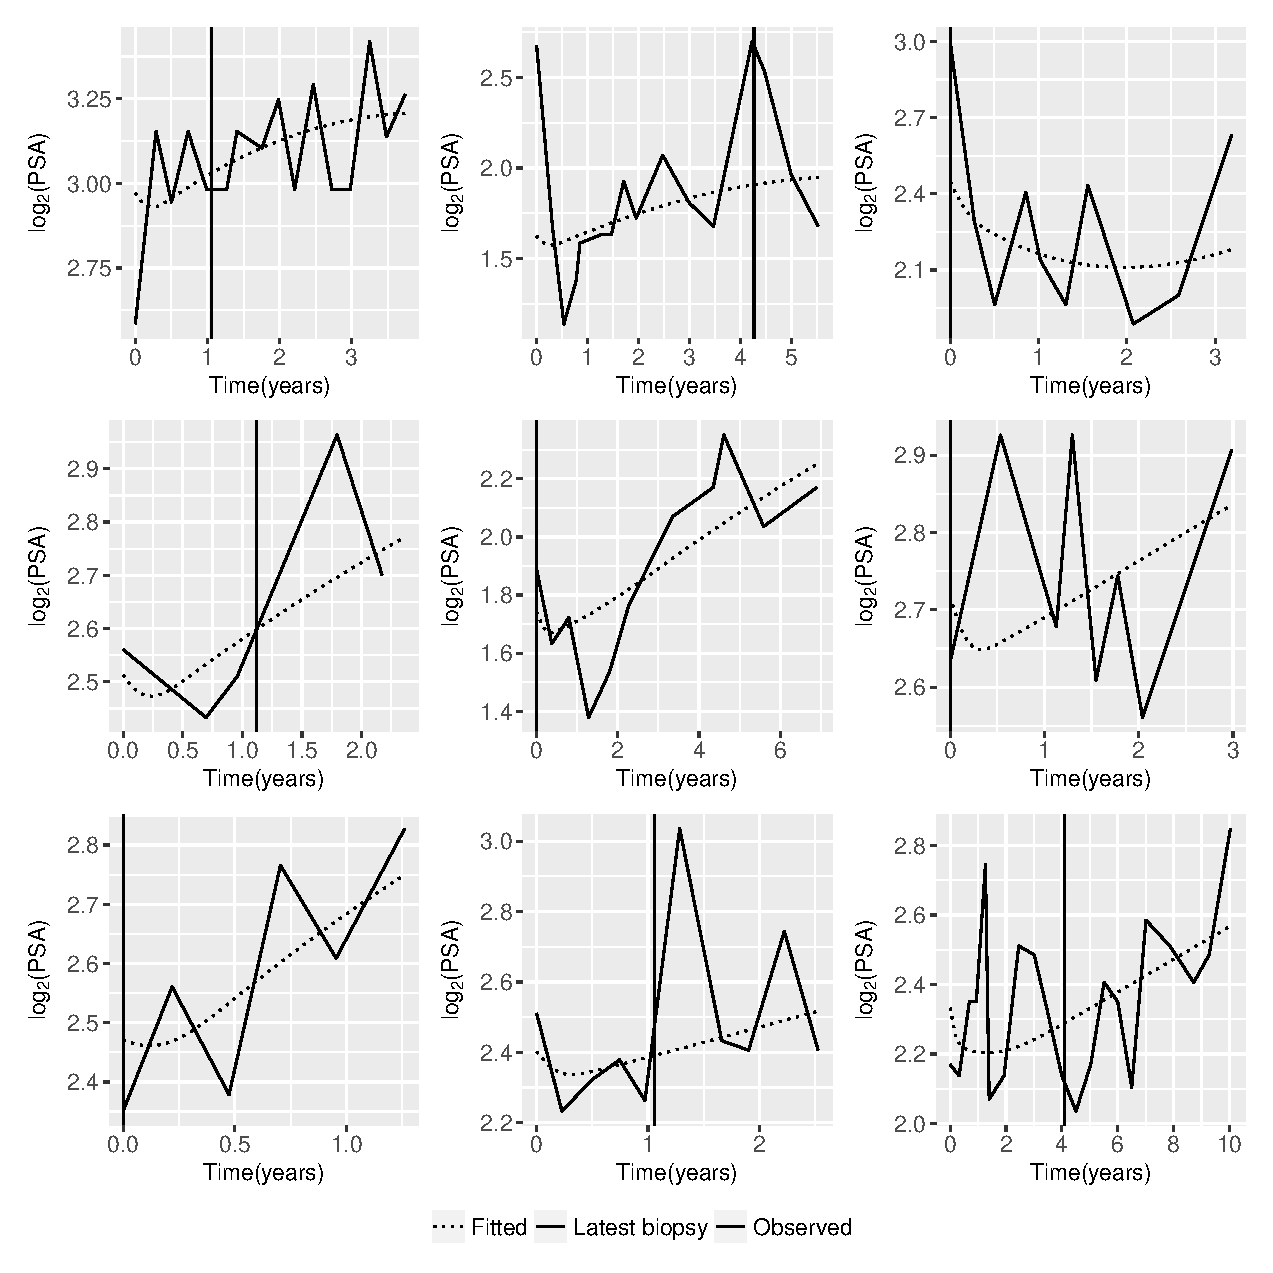
\includegraphics[width=\columnwidth]{images/model_fit/subject_fittedVsObserved_psa_t3.eps}}
	\caption{Fitted versus observed $\log_2 \mbox{PSA}$ profiles for nine randomly selected PRIAS patients. The fitted profiles utilize information from both the observed PSA levels and time of latest biopsy.}
	\label{fig : subject_fittedVsObserved_psa_t3}
	\end{figure}

\begin{table}[!htb]
\begin{center}
\caption{Estimated mean and 95\% credible interval for the parameters from the longitudinal sub-model of the joint model fitted to the PRIAS dataset.}
\label{tab : PSA_long}
\begin{tabular}{lrrrrr}
\Hline
Variable & Mean   & Std. Dev           & 2.5\%               & 97.5\%              & P              \\ \hline
Intercept                            &  2.412 & 0.012 & 2.388 & 2.435               & \textless0.000 \\
$(\mbox{Age} - 70)$                         & 0.003 & 0.001 & -3.039 $\times 10^{-4}$ & 0.005 & 0.084          \\
$(\mbox{Age} - 70)^2$       & -0.001 & 0.001 & -0.001 & -3.696 $\times 10^{-4}$ & \textless0.000 \\
Spline: visit time {[}0.0, 0.1{]} years   & 0.044 & 0.010 & 0.026 & 0.063 & \textless0.000 \\
Spline: visit time {[}0.1, 0.5{]} years & 0.297 & 0.015  &0.269 & 0.328           & \textless0.000 \\
Spline: visit time {[}0.5, 4.0{]} years & 0.316 & 0.025 &  0.270 & 0.364        & \textless0.000 \\
Spline: visit time {[}4.0, 7.0{]} years   & 0.466 & 0.032 & 0.402 & 0.527               & \textless0.000 \\
$\sigma$                               & 0.181 & 0.001 & 0.179 & 0.183              &  \\ \hline
\end{tabular}
\end{center}
\end{table}

\clearpage

For the relative risk sub-model, the parameter estimates in \ref{tab : PSA_survival} show that $\log_2 \mbox{PSA}$ velocity and the age at the time of inclusion in AS are strongly associated with the hazard of GR. For any patient, an increase in $\log_2 \mbox{PSA}$ velocity from -0.104 to 0.140 (first and third quartiles of the fitted velocities, respectively) corresponds to a 2.022 fold increase in the hazard of GR. An increase in age at the time of inclusion in AS from 65 years to 75 years (first and third quartiles of age in PRIAS dataset) corresponds to a 1.419 fold increase in the hazard of GR.

\begin{table}[!htb]
\begin{center}
\caption{Estimated mean and 95\% credible interval for the parameters of the relative risk sub-model of the joint model fitted to the PRIAS dataset.}
\label{tab : PSA_survival}
\begin{tabular}{lrrrrr}
\Hline
Variable                      & Mean   & Std. Dev & 2.5\%  & 97.5\%                 & P              \\ \hline
$(\mbox{Age} - 70)$                    & 0.035 & 0.006 & 0.023 & 0.047                  & \textless0.000 \\
$(\mbox{Age} - 70)^2$   & -0.001 & 0.001 & -0.003 & 1.364 $\times 10^{-4}$ & 0.084          \\
$\log_2 \mbox{PSA}$                  & -0.004 & 0.060 & -0.119 & 0.117 & 0.934         \\
Slope($\log_2 \mbox{PSA}$)           & 2.888 & 0.290 & 2.318 & 3.452 & \textless0.000 \\
\hline
\end{tabular}
\end{center}
\end{table}

\clearpage

To compare the predictive performance of a model having association between hazard of GR and $\log_2 \mbox{PSA}$ values, versus a model having the association with both $\log_2 \mbox{PSA}$ value and velocity, we calculate the area under the receiver operating characteristic curves, also called AUC \citep*{landmarking2017}, for these models. Since in a joint model time dependent AUC is more relevant, we calculate the AUC at year one, year two and year three of follow-up in AS. The time window for which the AUC is calculated is one year. The resulting AUC are presented in \ref{tab : AUC}.

\begin{table}[!htb]
\begin{center}
\caption{Area under the receiver operating characteristic curves (AUC), and 95\% confidence interval in brackets. AUC's are calculated for two joint models: first one having association between hazard of GR and $\log_2 \mbox{PSA}$ value as well as velocity, and second one having association with only $\log_2 \mbox{PSA}$ value.}
\label{tab : AUC}
\begin{tabular}{rrr}
\Hline
Year                      & $\log_2 \mbox{PSA}$ value and velocity association & $\log_2 \mbox{PSA}$ value association\\ 
\hline
1 & 0.613 [0.582, 0.632] & 0.595 [0.565, 0.618]\\
2 & 0.648 [0.608, 0.685] & 0.609 [0.568, 0.654]\\
3 & 0.593 [0.560, 0.638] & 0.590 [0.536, 0.628]\\
\hline
\end{tabular}	
\end{center}
\end{table}

\clearpage
\subsection{PSA-DT Dependent Interval Censoring in Time of Gleason Reclassification}
In PRIAS, the interval $l_i < T_i^* \leq r_i$ in which GR is detected depends on the observed PSA values (via PSA-DT). It is natural to question in this scenario if the parameters of the joint model are affected by PSA-DT dependent interval censoring. To this end, we discussed via the formulation of the likelihood function in \ref{subsec : int_censoring_fulllikelihood_proof}, that the joint model gives consistent and asymptotically unbiased estimates of the parameters even if the interval censoring depends on PSA-DT, under the condition that the model is correctly specified. However, in this section we also demonstrate this via a simulated dataset of 750 patients. The true event times $T^*_i$ for these patients were generated using parameters from a joint model fitted to the PRIAS dataset. However this joint model did not include association between velocity of log PSA values and hazard of GR. That is, the hazard of GR $h_i(t)$ at any time $t$ depends only on the underlying log PSA value $m_i(t)$ at that time. Furthermore, for these patients we used the schedule of PRIAS to generate the interval $l_i \leq T^*_i \leq r_i$ in which GR is detected. Thus the observed data for $i$-th patient is $\{\boldsymbol{y}_i, l_i, r_i\}$. Our aim is to show that if there is no association between $h_i(t)$ and velocity of log PSA value $m'_i(t)$, then even though the biopsy schedule depends on PSA-DT (which is a crude measure of PSA velocity), a joint model fitted with both value and velocity associations will have an insignificant velocity association. In the fitted joint model we found the value association (95\% credible interval in brackets) to be 0.182 [0.090, 0.274], and the velocity association to be -0.001 [-0.295, 0.254]. That is even though the schedule of biopsies depended upon observed PSA values it did not lead to a spurious velocity association. To check if we correctly specified the joint model, we performed several sensitivity analysis in our model (e.g., changing the position of the knots, etc.) to investigate the fit of the model and also the robustness of the results. In all of our attempts, the same conclusions were reached, namely that the $\log_2 \mbox{PSA}$ velocity is more strongly associated with the hazard of GR compared to the $\log_2 \mbox{PSA}$ levels.
\clearpage
% !TEX root =  ../supplementary.tex
\section{Simulation Study}
In the simulation study, we evaluated the following biopsy schedules: biopsy every year (annual), biopsy according to the PRIAS schedule (PRIAS), personalized biopsy schedules based on two fixed risk thresholds, namely, $\kappa=10\%$, and automatically chosen $\kappa^*(v)$ (Section~3 of main manuscript), and automatically chosen ${\kappa^*\{v \mid E(D)\leq 0.75\}}$ with a constraint of 0.75 years (9 months) on expected delay in detecting progression. The choice of 0.75 years delay constraint is arbitrary and is only used to illustrate that applying the constraint limits the average delay at 0.75 years.  We compare all the aforementioned schedules on two criteria, namely the number of biopsies they schedule and the corresponding time delay in detection of cancer progression, in years (time of positive biopsy - true time of cancer progression). The corresponding results, using ${\mbox{500} \times \mbox{250}}$ test patients are presented in~\ref{table:sim_study_all}. Since the simulated cohorts are based on PRIAS, roughly only 50\% of the patients progress in the ten year study period. While, we are able to calculate total number of biopsies scheduled in all $500 \times 250$ test patients, but the time delay in detection of progression is available only for those patients who progress in ten years (\textit{progressing}). Hence, we show the simulation results separately for \textit{progressing} and \textit{non-progressing} patients.

\begin{table}[!htb]
\caption{\textbf{Simulation study results for all patients}: Estimated mean ($\mu$), median (Med), first quartile $\mbox{Q}_1$, and third quartile $\mbox{Q}_3$ for number of biopsies (nb) and for the time delay (d) in detection of cancer progression in years, for various biopsy schedules. The delay is equal to the difference between the time of the positive biopsy and the simulated true time of progression. Types of schedules: ${\kappa=10\%}$ and $\kappa^*(v)$ schedule a biopsy if the cumulative-risk of cancer progression at a visit is more than 10\%, and an automatically chosen threshold, respectively. Schedule ${\kappa^*\{v \mid E(D)\leq 0.75\}}$ is similar to $\kappa^*(v)$ except that the euclidean distance is minimized under the constraint that expected delay in detecting progression is at most 9 months (0.75 years). Annual corresponds to a schedule of yearly biopsies, and PRIAS corresponds to biopsies as per PRIAS protocol.}
\label{table:sim_study_all}
\begin{tabular}{l|rrrr|rrrr}
\hline
\hline
\multicolumn{9}{l}{\textbf{Progressing patients (50\%)}}\\
\hline
Schedule & $\mbox{Q}_1^{\mbox{nb}}$ & $\mu^{\mbox{nb}}$ & $\mbox{Med}^{\mbox{nb}}$ & $\mbox{Q}_3^{\mbox{nb}}$ & $\mbox{Q}_1^{\mbox{d}}$ & $\mu^{\mbox{d}}$ & $\mbox{Med}^{\mbox{d}}$  & $\mbox{Q}_3^{\mbox{d}}$ \\
\hline
Annual        & 1  & 3.71 & 3  & 6  & 0.29 & 0.55 & 0.57 & 0.82\\
PRIAS         & 1  & 2.88 & 2  & 4  & 0.38 & 0.92 & 0.74 & 1.00\\
$\kappa=10\%$ & 1  & 2.55 & 2  & 4  & 0.45 & 1.00 & 0.85 & 1.33\\
$\kappa^*(v)$ & 1  & 2.46 & 2  & 3  & 0.45 & 0.89 & 0.86 & 1.26\\
$\kappa^*\{v \mid E(D)\leq 0.75\}$ & 1  & 3.39 & 3  & 5  & 0.32 & 0.61 & 0.63 & 0.88\\
\hline
\multicolumn{9}{l}{\textbf{Non-progressing patients (50\%)}}\\
\hline
Annual         & 10 & 10.00   & 10 & 10 & - & - & - & -\\
PRIAS          & 4  & 6.40 & 6  & 8  & - & - & - & -\\
$\kappa=10\%$  & 4  & 4.91 & 5  & 6  & - & - & - & - \\
$\kappa^*(v)$  & 6  & 6.22 & 6  & 7  & - & - & - & -\\
$\kappa^*\{v \mid E(D)\leq 0.75\}$ & 8 & 8.68 & 9  & 9  & - & - & - & -\\
\hline
\end{tabular}
\end{table}
\clearpage
% !TEX root =  ../supplementary.tex
\section{Source Code}
The R code for fitting the joint model to the PRIAS dataset, and for the simulation study are available at \url{https://github.com/anirudhtomer/prias/tree/master/src/decision_analytic}. We refer to this location as `DATA\_HOME' in the rest of this document.

\subsection{Fitting the joint model to the PRIAS dataset}
\textbf{Accessing the dataset:}
The PRIAS dataset is not openly accessible. However, access to the database can be requested via the contact links at \url{www.prias-project.org}.\\

\textbf{Formatting the dataset:}
This dataset however is in the so-called wide format and also requires removal of incorrect entries. This can be done via the R script \url{DATA_HOME/fittingModel/dataset_cleaning.R}. This will lead to two R objects, namely `prias.id' and `prias\_long'. The `prias.id' object contains information about time of cancer progression for PRIAS patients. The `prias\_long' object contains longitudinal PSA, DRE measurements, time of biopsies and results of biopsies.\\

\textbf{Fitting the joint model:}
We use a joint model for time to event and bivariate longitudinal data to model the evolution of PSA and DRE measurements over time, and to simultaneously model their association with the risk of cancer progression. The R package we use for this purpose is called \textbf{JMbayes} (https://cran.r-project.org/web/packages/JMbayes/JMbayes.pdf). The API we use, however, are currently not hosted on CRAN, and can be found here:
\url{https://github.com/drizopoulos/JMbayes}. The joint model can be fitted via the script \url{DATA_HOME/fittingModel/psa_dre_jointAnalysis.R}. It takes roughly 6 hours to run on an Intel core-i5 machine with 4 cores, and 8GB of RAM. 

The graphs presented in the main manuscript, and the supplementary material can be generated by the scripts \url{DATA_HOME/fittingModel/demographs.R}, and \url{DATA_HOME/fittingModel/modelDiagnostic.R}, respectively.

\subsection{Running the simulation study}
The simulation study can be run by the following script: \url{DATA_HOME/simulationStudy/controller.R}. Although it depends on other files, the code should run without errors as long as the directory structure is maintained. An entire simulation study may take weeks to run. However, this can be controlled via the variable `dataSetNums' in the script. Graphs related to simulation study results can be generated from the scripts \url{DATA_HOME/simulationStudy/decisionMakingGraph.R} and \url{DATA_HOME/simulationStudy/produceResults.R} 
\clearpage
\printbibliography

\appendix

\end{document}